\documentclass{beamer}
\usepackage[utf8]{inputenc}

\usetheme{Madrid}
\usecolortheme{default}
\usepackage{amsmath,amssymb,amsfonts,amsthm}
\usepackage{txfonts}
\usepackage{tkz-euclide}
\usepackage{listings}
\usepackage{adjustbox}
\usepackage{array}
\usepackage{tabularx}
\usepackage{gvv}
\usepackage{lmodern}
\usepackage{circuitikz}
\usepackage{tikz}
\usepackage{graphicx}

\setbeamertemplate{page number in head/foot}[totalframenumber]

\usepackage{tcolorbox}
\tcbuselibrary{minted,breakable,xparse,skins}



\definecolor{bg}{gray}{0.95}
\DeclareTCBListing{mintedbox}{O{}m!O{}}{%
  breakable=true,
  listing engine=minted,
  listing only,
  minted language=#2,
  minted style=default,
  minted options={%
    linenos,
    gobble=0,
    breaklines=true,
    breakafter=,,
    fontsize=\small,
    numbersep=8pt,
    #1},
  boxsep=0pt,
  left skip=0pt,
  right skip=0pt,
  left=25pt,
  right=0pt,
  top=3pt,
  bottom=3pt,
  arc=5pt,
  leftrule=0pt,
  rightrule=0pt,
  bottomrule=2pt,
  toprule=2pt,
  colback=bg,
  colframe=orange!70,
  enhanced,
  overlay={%
    \begin{tcbclipinterior}
    \fill[orange!20!white] (frame.south west) rectangle ([xshift=20pt]frame.north west);
    \end{tcbclipinterior}},
  #3,
}
\lstset{
    language=C,
    basicstyle=\ttfamily\small,
    keywordstyle=\color{blue},
    stringstyle=\color{orange},
    commentstyle=\color{green!60!black},
    numbers=left,
    numberstyle=\tiny\color{gray},
    breaklines=true,
    showstringspaces=false,
}
\begin{document}

\title 
{4.3.23}
\date{September 14,2025}


\author 
{Kishora Karthik-EE25BTECH11034}
\frame{\titlepage}
\begin{frame}{Question}
The line segment joining the points $\vec{A}(3,2)$ and $\vec{B}(5,1)$ is divided at the point $\vec{P}$ in the ratio $1:2$ which lies on $3x - 18y+k=0$. Find the value of k.\\
\end{frame}

\begin{frame}{ Solution}
Given the points,
\begin{align}
    \vec{A}=\begin{myvec}{3\\2}\end{myvec}\\ 
    \vec{B}=\begin{myvec}{5\\1}\end{myvec}
\end{align}
and the line $L_1$,
\begin{align}
    L_1: \myvec{3 & -18}\vec{x} = -k
\end{align}
\begin{align}
    \implies \vec{n}^{\top}\vec{x}=0
\end{align}
Where,
\begin{align}
     \vec{n}=\myvec{3\\-18}
\end{align}
\end{frame}

\begin{frame}{Solution}
Let the vector $\vec{P}$ be a point on the line $3x - 18y+k=0$ wihch divides the line segment joining the points $\vec{A}$ and $\vec{B}$.
\\\\
Section formula for a vector $\vec{P}$ which divides the line formed by vectors $\vec{A}$ and $\vec{B}$ in the ratio $k:1$ is given by
\begin{align}
    \vec{P}=\frac{k\vec{B}+\vec{A}}{k+1}
\end{align}
\begin{align}
    \vec{P}=\myvec{\vec{A} & \vec{B}}\myvec{\frac{1}{k+1}\\\frac{k}{k+1}}
\end{align}
Here, $k=1/2$.
\begin{align}
    \implies \vec{P}=\myvec{\vec{A} & \vec{B}}\myvec{\frac{2}{3}\\\frac{1}{3}}
\end{align}\\
\end{frame}
\begin{frame}{Solution}
Since $\vec{P}$ lies on line $L_1$,
\begin{align}
    \vec{n}^{\top}\vec{P}=0
\end{align}
\begin{align}
    \implies \myvec{3 &-18}\myvec{\vec{A} & \vec{B}}\myvec{\frac{2}{3}\\\frac{1}{3}}=-k
\end{align}
\begin{align}
    \implies \myvec{3 & -18}\myvec{3 & 5\\2 & 1}\myvec{\frac{2}{3}\\\frac{1}{3}}=-k
\end{align}
\end{frame}
\begin{frame}{Solution}
\begin{align}
    \implies \myvec{3\cdot 3 + (-18)\cdot 2 & 3\cdot 5 + (-18)\cdot 1}\myvec{\frac{2}{3}\\\frac{1}{3}}=-k
\end{align}
\begin{align}
    \implies \myvec{-27&-3}\myvec{\frac{2}{3}\\\frac{1}{3}}=-k
\end{align}
\begin{align}
    \implies \myvec{(-27)\cdot \frac{2}{3} + (-3)\cdot \frac{1}{3}}=-k
\end{align}
\begin{align}
    \implies k=19
\end{align}
$\therefore$ The value of k is 19 and the equation of the line is $3x - 18y+19=0$.   
\end{frame}
\begin{frame}{Plot}
    \centering
    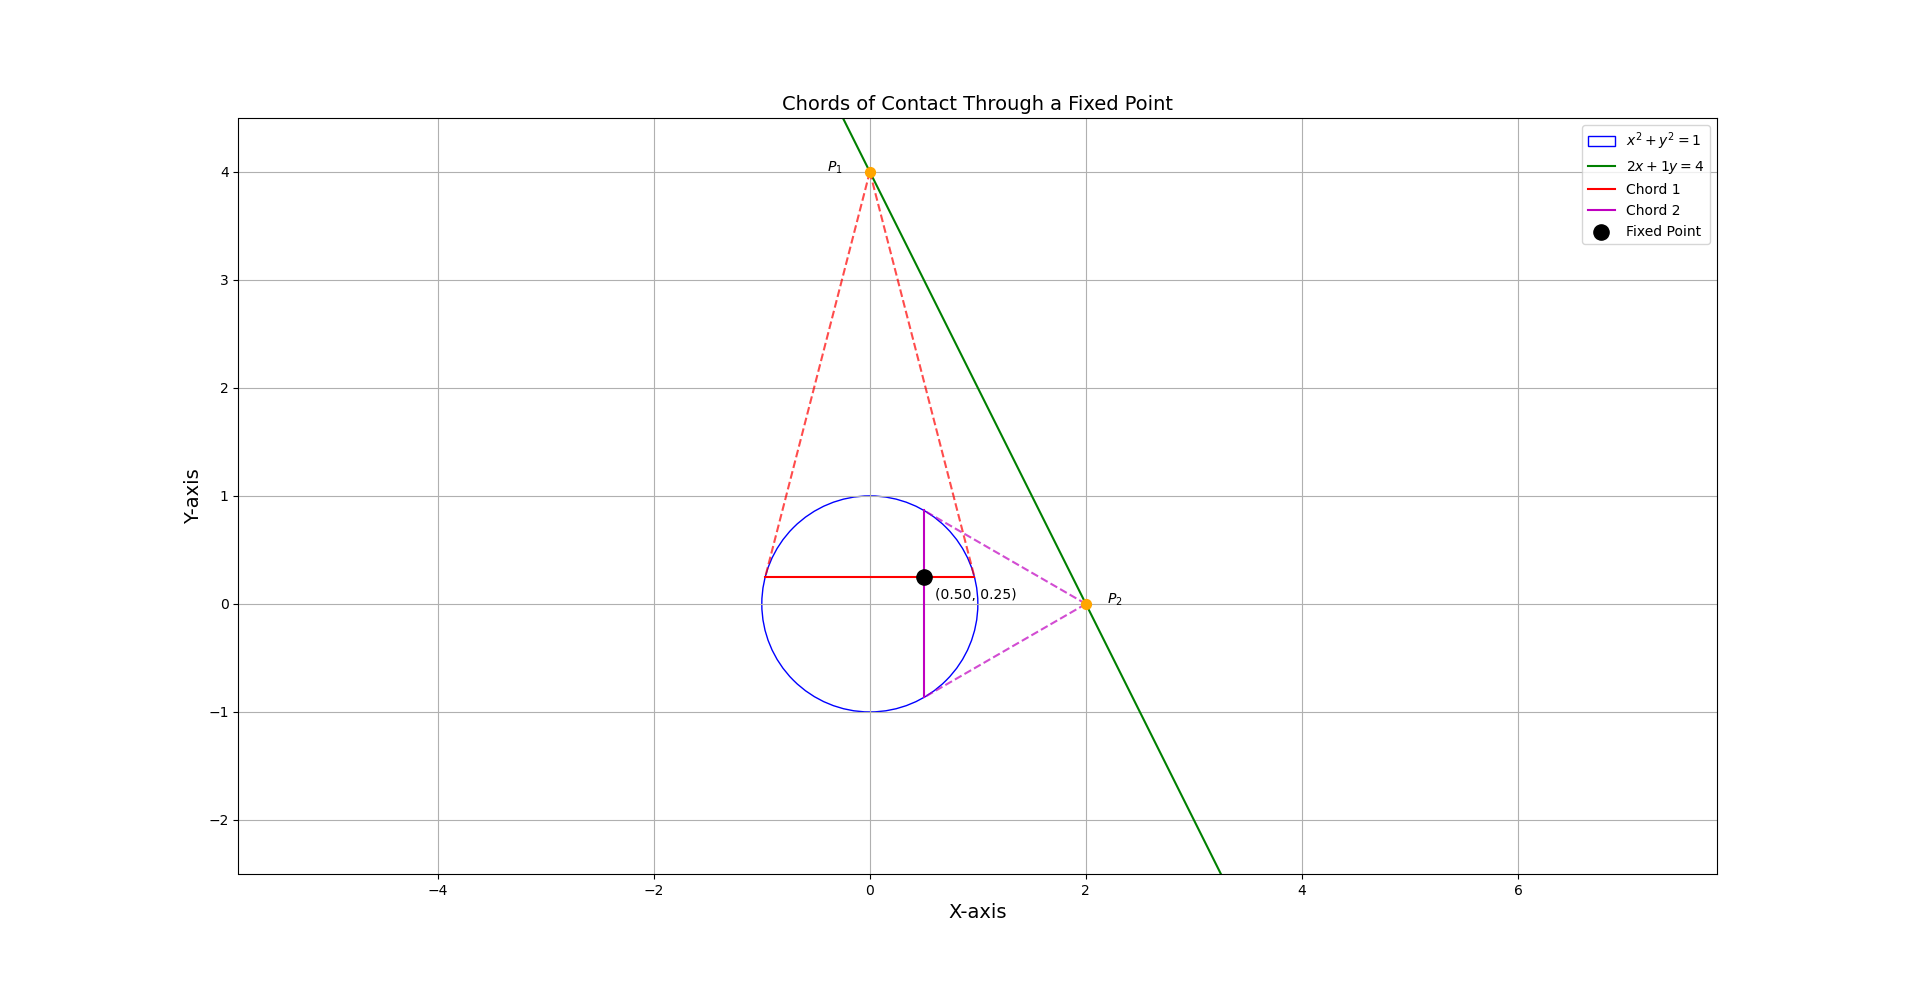
\includegraphics[width=\columnwidth, height=1\textheight, keepaspectratio]{figs/fig1.png} 
\end{frame}

\end{document}



